\documentclass{article}
\usepackage[margin=1.5cm]{geometry} % Change the margins
\usepackage[utf8]{inputenc} % - Defines what coding LaTeX uses. Use this one.
\usepackage[english]{babel}
\usepackage[T1]{fontenc}
\usepackage{graphicx} % - Package for including images in the document.
\usepackage{amsmath}
\usepackage{mathtools}
\usepackage{float}
\usepackage{caption} % Correct spacing for captions
\usepackage{siunitx} % Package for handling numbers (ex \num{1e6}), units (ex \SI{15,3}{Nm}) and intervals (ex\SIrange{10}{20}{\celcius}) correctly
\usepackage{appendix}
\usepackage{hyperref}
\usepackage{datetime}

\usepackage[style=numeric,backend=biber,sorting=none]{biblatex}
\DeclareLanguageMapping{english}{english-apa}
\addbibresource{references.bib}
\nocite{*}

\newdateformat{monthyeardate}{%
  \monthname[\THEMONTH], \THEYEAR}

\title{SysML 2.0 Viewer in a Browser}
\author{Oliver Högberg, \tt olihgb-7@student.ltu.se \\ 
Emma Carlsson, \tt emacar-8@student.ltu.se \\ 
Axel Kärnebro, \tt axekrn-7@student.ltu.se \\ 
Magnus Stenfelt, \tt magset-8@student.ltu.se \\
\\
\\
\\
\\
\\
\\
\\
\\
\\
\\
\includegraphics[width=0.3\textwidth]{ltu_swe.jpg}}
\date{\monthyeardate\today}


\begin{document}

\maketitle
\newpage
\tableofcontents
\newpage

\section{Introduction}

\subsection{Background}
When developing large and complex systems it is very important not to lose understanding of the system, however this can be quite a challenge. This is why developers have used some kind of modelling language throughout time. Modelling languages allow for creation of a graphical representation of the system, with varying levels of detail and complexity depending on what the project in question needs. It also allows developers to create and plan the entire system ahead of time, making it easier to avoid messy implementations and improves overall readability. UML \cite{UML}, Unified Modeling Language, is one such language and SysML \cite{SysML}, Systems Modeling Language, is an extension of UML which lets users practice Model-Based Systems Engineering \cite{MBSE} (MBSE).
\\ \\
The first iteration of SysML is a complete modelling language with very useful tools for creating and viewing system models. It is also a graphical modeling language meaning it consists of different types of diagrams which contain information useful for conveying system structures. There is now a new iteration of SysML called SysML v2 which is a purely textual modeling language meaning SysML v2 looks more like a programming language. This creates a problem where less tech-literate users have a very hard time understanding SysML v2 as it has a very steep learning curve and the systems are very hard to visualize. To make SysML v2 more palpable for users of varying technical proficiency tools need to be developed to translate the SysML v2 text to diagrams. There are some tools that accomplish this to some degree, such as Eclipse Papyrus \cite{EclipsePapyrus}, but they are very complicated to install and use making them unsuitable for less tech-literate users.
\\ \\
A proof of concept of an interactive SysML v2 web viewer has been developed in a bachelor thesis at LTU where Jesper Nilsson \cite{Jesper2020} proved that it is possible to render SysML diagrams in a browser. Tommy Andersson \cite{Tommy2020} would later continue the project by building on the proof of concept as a summer job, however it was discovered that a proof of concept does not necessarily scale and their solution could not be developed any further. Additional work is required to restart the project from scratch to avoid these scalability issues. 
\\ \\
This is why this current iteration of the project was started, to find a way around the issues that the prior project iterations arrived at and to create a strong foundation towards a finished product; an interactive SysML v2 viewer in a browser.

\subsection{Problem description}
%%Uppdaterad efter Jans feedback kan behöva mer arbete
The task is to create a web viewer for SysML v2. Web viewer in this case means a web-based application to which we can upload the SysML v2 files which then displays interactive SysML diagrams inside of a web-browser. The web viewer is supposed to be used by a system designer to create a clearer and easier to understand description of a complex system. In order to accomplish this the application needs to be able to display the diagrams included in SysML v2 based on a input file in the format of a .sysml file. After creating the .sysml file, it will be uploaded to the application and shown as a SysML v2 diagram in a clear and interactive manner. The final product is supposed to have support for a user to: interact with the diagram views; click SysML objects to get to other diagram views and to view specific SysML object functionality.
\\\\
The goal of this project is get an understanding of the SysML v2 language to create an easy to use tool to display future SysML diagrams. Another very important goal, if not the main goal itself, is to create the application in such a way that it can be built upon by other developers in the case of this project not completing the first mentioned goal. The application also has to be able to be built upon due to SysML v2 not being finished and it still being updated. To summarize this to one sentence the project is to create a scalable SysML v2 web viewing tool that is easy to use and understand.

\subsection{Objectives}
The overall objective with this project is to create a tool that allows the user to get a clear understanding of a complex system. This tool should be able to give both an overview of the system and show the small details and how all the parts are connected. The systems provided to the tool should be visualized using the SysML diagrams and written with the syntax of SysML v2 which is still in development. A very important part of this project is to make it open and scalable, our main goal is to lay the groundwork so that others can build upon and perfect it. 
\\\\
This shall be demonstrated at the end of the project by running an example project written in SysML v2 on our application which should be able to parse the code, display at least one diagram and be interactive in such a way that the user can navigate from one diagram view to another. This diagram should be either a block definition diagram, internal block diagram or a sequence diagram. 
\\\\
To reach this objective we need to make sure that we, as developers really understand what we are creating and that we have a sound and well thought through plan to avoid getting stuck. We also need to use the former attempts at this project to learn what worked and what to do differently in order to succeed.

\section{System design}\label{sec:system_design}

\begin{figure}[H]
    \begin{center}
        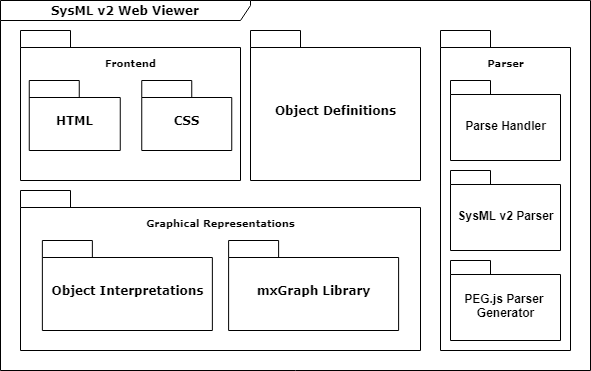
\includegraphics[width=0.8\textwidth]{Module_diag-SysML_project.png}
        \caption{Package diagram describing the basic structure of the implementation}
        \label{package}
    \end{center}
\end{figure}
The package diagram in figure \ref{package} shows the overall structure of the application. It consists of a front-end module, an object definitions module, a parser module and a graphical representations module. The front-end module is used to display a website based application using basic HTML \cite{HTML} and CSS \cite{CSS} documents to present a graphical view of a system using SysML v2. 
\\\\
The object definitions module consists of predefined SysML v2 object definitions based on the SysML v2 syntax. These are the objects that the entire application utilize when handling the SysML v2 building blocks and diagrams. The object definitions together with the parser module is then used by the graphical representations module to provide a graphical output of the parsed input.
\\\\
The parser module in itself consists of the PEG.js parser generator \cite{PEG-JS}, parse handler and the SysML v2 parser. The PEG.js parser generator is used together with a grammar rule-set to generate the SysML v2 parser, which is a functional PEG parser \cite{wiki:PEG}. The parse handler connects the SysML v2 parser with the object definitions so that the parse handler can create SysML v2 objects based on the parsed input. 
\\\\
The graphical representations module consists of the object interpretations used to visualize the actual SysML v2 objects created from the parse handler based on the object definitions. The graphical representations module also consists of the mxGraph library \cite{mxGraph} used as the library to display graphics in the application. 

\begin{figure}[H]
    \begin{center}
        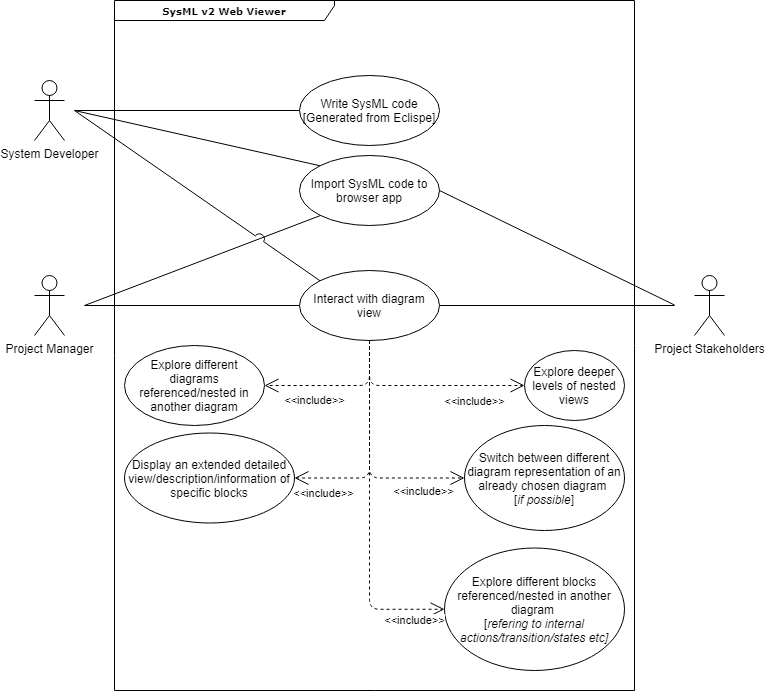
\includegraphics[width=0.8\textwidth]{Use-case_SysMLProject.png}
        \caption{Use-case diagram describing some uses in the the application}
        \label{use-case}
    \end{center}
\end{figure}
The use-case diagram shown in figure \ref{use-case} describes some of the various uses that the application is planned to have in the future, since these uses unfortunately did not get implemented during this projects time frame. The primary actors for the application are: 
\begin{itemize}
  \item System Developer - The main function of this actor is as a developer and engineer of a particular system. 
  \item Project Manager - This actors main function is as the project lead of the particular system that is being developed. As a project manager this actor oversees the team of system developers and provides the communication channel with the project stakeholders.
  \item Project Stakeholders - This actors main function is that of an external (or in some cases internal) party which have interests of the particular system being developed. This actor can in a sense be seen as the customer of the particular system being developed.
\end{itemize}

\begin{figure}[H]
    \begin{center}
        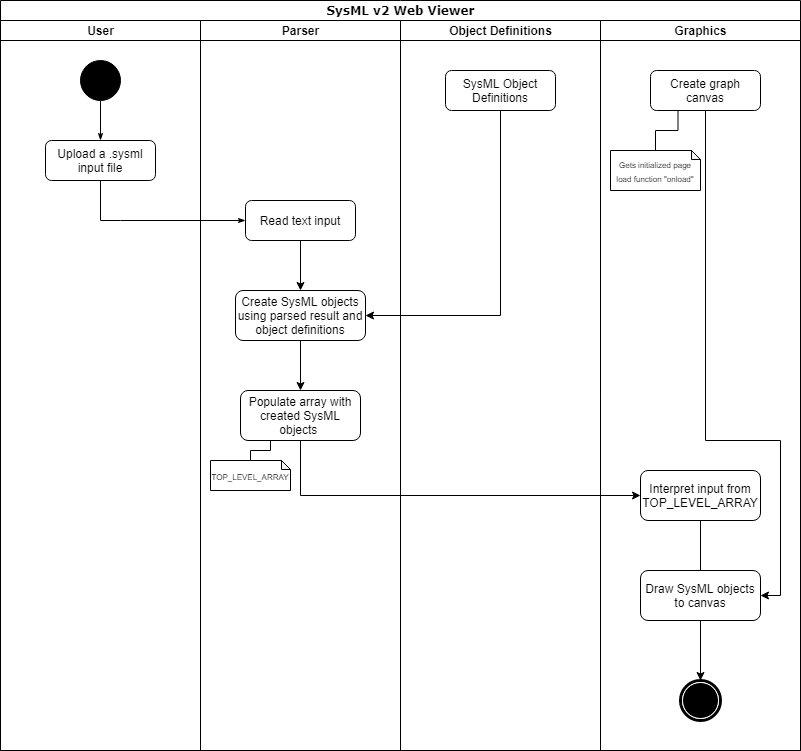
\includegraphics[width=0.8\textwidth]{Activity_diag-SysML-project.png}
        \caption{Activity diagram showing the use of the application}
        \label{activity}
    \end{center}
\end{figure}
The activity diagram in figure \ref{activity} shows the general functionality of the application as one of the actors presented earlier uses the application. The process describes the general actions taken in the application from the point of a user uploading a .sysml file. As shown in the figure the basic process of handling an input file is rather simple in that the actions taken by the application does not involve to many steps to produce a complete result. 


\newpage
\section{Results}

\subsection{Delivery}
%Beskrivning av vad som levereras av projektet i relation till ursprunglig uppgift och mål (kap. 1.3). Beskrivningen ska koppla till uppdaterade designbeskrivningar i Kap. 2, dvs. förklara till vilken grad det som implementerats, testats och demonstrerats har realiserat det som beskrivs med designen. Därtill ska en förklaring ges av hur designen realiserats (t.ex. med vilka programpaket/bibliotek), hur mogna olika delar kan anses vara, samt vad som inte har realiserats. 

\begin{figure}[H]
    \centering
    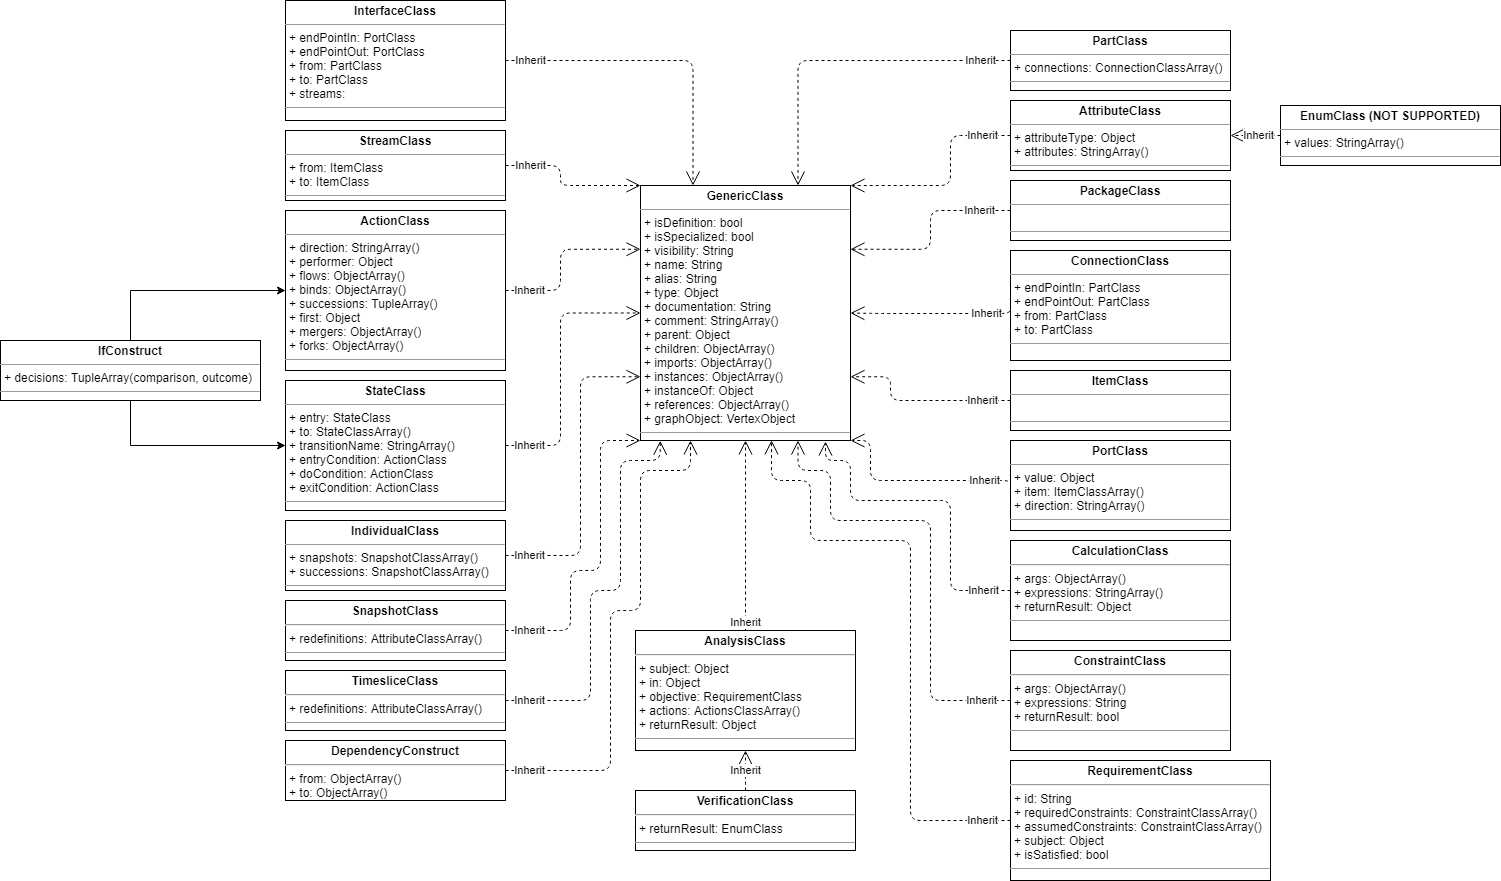
\includegraphics[width=\textwidth]{Class_diagram-SysMLv2.png}
    \caption{The planned class diagram for the current and future SysML v2 object definitions}
    \label{fig:class_diagram}
\end{figure}
The first part of the project was all about planning as into the future as possible. The entire first sprint, which in the case of the project was a development period of around 3-4 weeks, and part of the second sprint was spent planning for implementation as far as we could. We read through the available SysML v2 documents and tried to fit all of the keywords used in SysML v2 into a class diagram. This diagram, shown in figure \ref{fig:class_diagram}, contains our understanding of SysML v2 and how we would need classes to look to implement SysML v2 functionality in JavaScript. This was created to try to make our development future proof and make it easy to continue for someone else after this project has ended.


\begin{figure}[H]
    \centering
    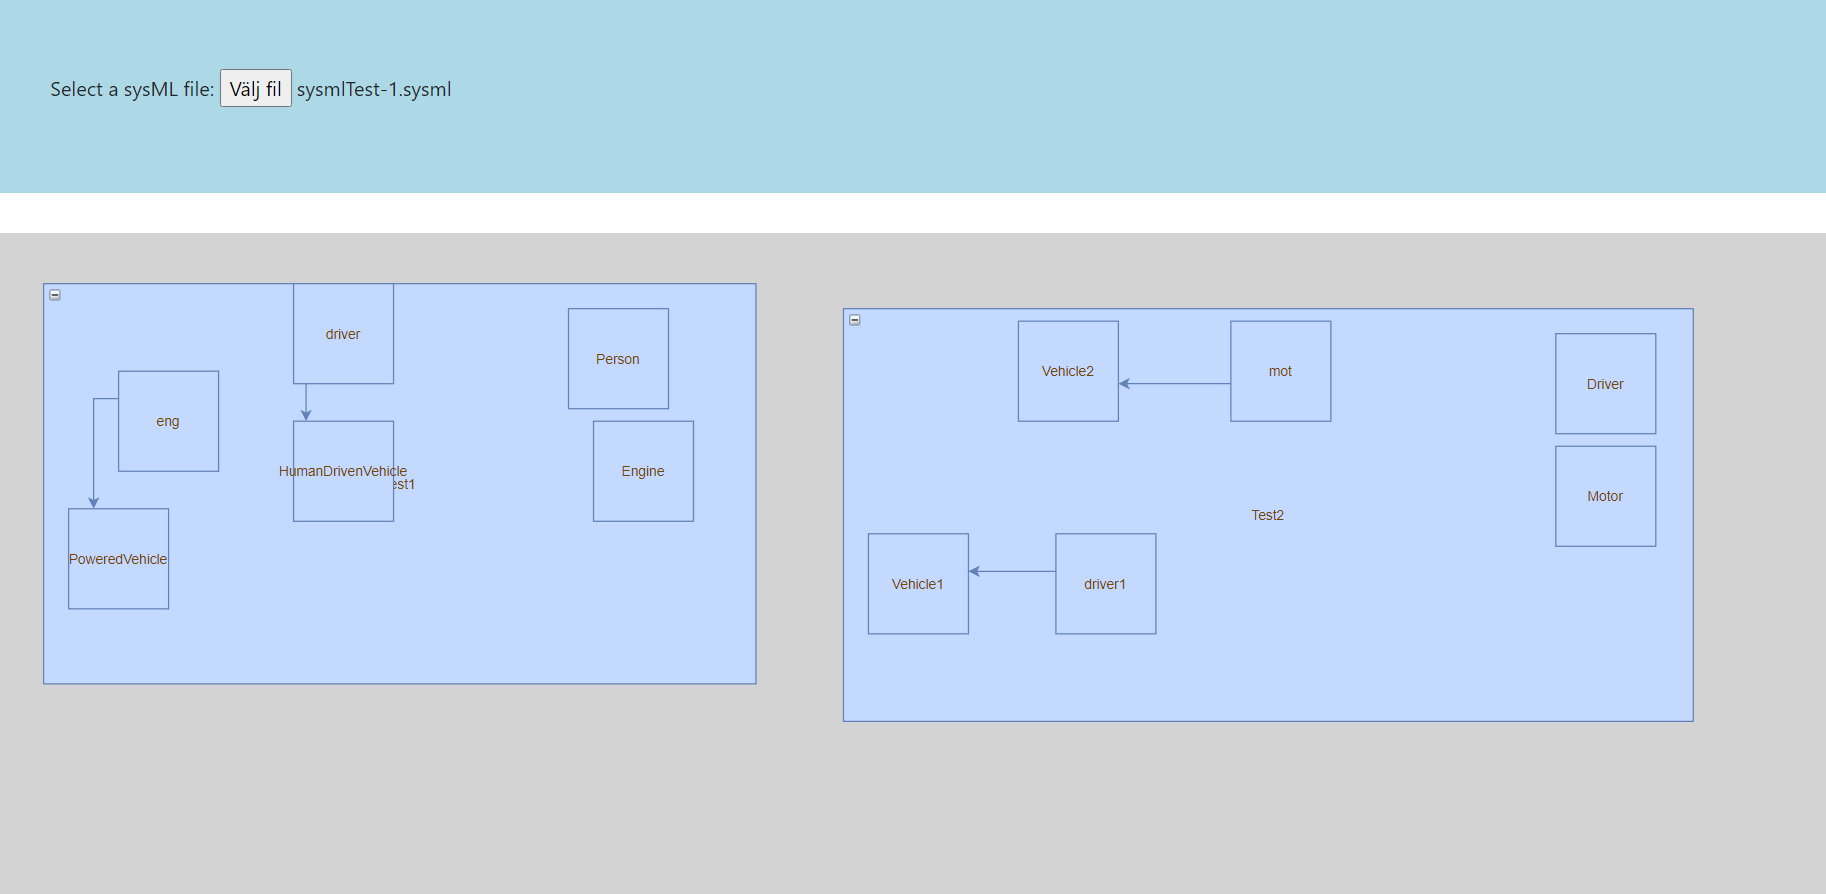
\includegraphics[width=\textwidth]{unknown.png}
    \caption{The current version of the application}
    \label{fig:my_label}
\end{figure}

The end product that we ended up with was a proof of concept rather than a fully fledged interactive SysML v2 web viewer. In its current state it is only possible to upload a .sysml file containing packages, part definitions and part usages and display them as crude diagrams in a restricted manner. The layout algorithm and placing of the different SysML objects is not implemented yet. There are also no official SysML diagrams that can be shown yet. However there are things that have been implemented that are very important and useful for future work. A parser generator, PEG.js mentioned earlier in section \ref{sec:system_design}, has been used to create a functional PEG parser which provides the basic groundwork regarding parsing for future development on this project and testing of the generator has shown that it is suitable for the task. A generalized foundation of object definitions used to create the SysML objects that can be used for graphical representation has also been created. 
\\\\
There are a few things that have not been incorporated into the parser at the moment. Specifically the things in the parser that are not yet fully realized and mature are the missing rule-sets for SysML objects other than packages, part definitions and part usages. There are several different functions, rules and more that has to be added for a functioning SysML parser. There is one issue that has been purposely ignored due to an assumption made on our part. What we chose to ignore was checking for errors in the code and assuming that it is correctly written. We can assume this because we expect the .sysml files to be written in the Eclipse IDE \cite{eclipseIDE} where there is a syntax checker already included for the SysML v2 language. 
\\\\
The graphical representation was created using a library called mxGraph \cite{mxGraph}. This part of the product is not as developed as most other parts, there were many functions that we wanted to implement but did not have time for. What we did implement is the very basic ability to draw objects based on information from the parser. It can draw nestled objects within each other but it can only draw the same looking rectangles for all objects, meaning that parts and packages look the same which they should not. Parts within parts are represented using arrows while parts within packages are nestled. When a file is uploaded all the objects are just drawn in the upper left corner stacked on each other instead of placed using a layout algorithm like we planned. While it is possible to move objects and arrows, it does not look good. Also it was supposed to be interactive which it is not at this point. 
\\\\
Most of the code and work put into the project has been in the effort to create a solid starting point for future attempts at this web viewer. That has been the goal of this project the entire time. In the end, the goal of this project was not a fully functioning SysML v2 web viewer. As such we did manage to succeed in delivering what was asked of us to deliver; a solid foundation to continue developing on. 

\subsection{Testing}

%Local - changes introduce new bugs.
%Unmasked - changes unmask previously existing bugs.
%Remote - Changing one part breaks another part of the program. For example, Module A writes to a database. Module B reads from the database. If changes to what Module A writes to the database break Module B, it is remote regression.

\subsubsection{Risk of regression}

Based off of an interview with Tommy Andersson who previously worked on this project, our design is aiming to be as modular as possible with very distinct and separated classes and methods to provide for the application to be as scalable as possible. This, of course, raises the risk for remote regression as a small change in a method may ripple across the entire program. For example we might need to change a method to make it more efficient or if we discover a bug and this seemingly small change could cause much bigger problems since other parts of the program depends on this method. 
\\\\
Due to the fact that the planned implementation of the diagrams involves implementing the diagram one at a time, a big risk of both unmasked and remote regression appears. For example, modifying the parsing code  to include new definitions of SysML v2 functions may unmask bugs that was previously harmless and in turn, the graphical representation might break when implementing these new diagram definitions as well. Creating new definitions can create remote regression in both the graphical representation and the parser as well as creating local regression risks and as such extra care will have to be put into handling new definitions.
\\\\
Every time we add something new there is of course also the risk of local regression, and when modifying existing classes and methods to account for new diagrams the risk of local regression also increases. The risk of unmasked regression also increases in these situations.
\\\\
Our design choices open up the possibility of many regression risks, however the trade off for us seems worth it due to the benefits of scalability and the ability to salvage code in the case of failure. Regression risks can be worked around through proper testing and vetting but scalability issues are not so easily patched at a later date.


\subsubsection{Strategy for regression testing}

\paragraph{Traceability}
From our use case diagram and requirement specifications we can decide what to test using traceability. For example the use case diagram describes that a user should be able to import SysML code to browser app and then interact with the diagrams. This could be tested to make sure that the functions works as intended and similarly this should be done for every use-case described. One approach to make sure that the tests are traceable is to use branches in the development of different parts of the application. This provides a way to easily trace tests to specific branches of code containing specific functionality.

\paragraph{Change analysis}
To ensure that no errors manages to sneak it is way past development, a close eye needs to be kept on any rippling effects after changes. What we mean by this is that a highly modular program becomes very hard to keep track of when the program scales to larger sizes and as such, remote regression becomes very hard to notice and patch. When we want to add or change a part we need to triple check all the parts that inherits what we changed to make sure that behaviour has not changed. We need to trace the changes all the way through all the other modules that it can affect to make sure our program works as intended.

\paragraph{Quality risk analysis}
The biggest factor in the success of this project is whether or not we can interpret the SysML v2 language and documentation correctly. A failure to understand the SysML v2 language and documentation would lead to a poor implementation of the application which would lead to an application that is unable to be built upon in the future. Therefor a strategy is to make up a solid plan of how the solution is supposed to be implemented and make it possible for others to build upon this plan in the future.

\paragraph{Cross functional testing}
Using cross functional testing we can find bugs in unexpected places. This is done by testing functions that should have no effect on each other both together and in isolation. If the results are different, there is a bug. At first we could do a wide search to cover large areas of the system in order to find common areas with bugs. Then when we know these problem areas, we can focus the testing on them to uncover more bugs. 

\newpage
\subsubsection{Development description}

The following table describes our plan for automated unit and system level testing for regression. Our plan contains two stories, one for unit level and one for system level, on how to create automated testing.

\begin{figure}[H]
    \begin{center}
        \includegraphics[width=1\textwidth]{Test-table.png}
        \caption{Table describing automated test stories}
        \label{test-strat}
    \end{center}
\end{figure}

\subsubsection{Test strategy}
%Beskrivning av hur testning skett i projektet, dels fortlöpande/kontinuerligt och dels inför demo/leverans. Beskrivningen ska beröra följande termer; ”traceability, change analysis, quality risk analysis and cross-functional testing” (dvs. samma termer som diskuteras i kap. 3.2.2). Beskrivningen ska kritiskt bedöma och beskriva vad som fungerat bra respektive vad som kunnat göras bättre beträffande testning i projektet. 

Our general strategy for testing has been to try every new function out locally and separate during development. Then try it out with other parts when merging to see if they are compatible. Due to our extensive planning this has worked quite well as everyone had a good understanding of the whole picture and how the parts were supposed to fit together. Also since we coded in pairs there was always someone to discuss with and who could help look for errors and bugs.
\\\\
Our strategy for traceability was implemented right before we started to code by creating branches in our Github, which can be found in the appendix. The code was not pushed to main branch until the very end when we had a finished product. During development our group split into pairs which each had a branch. The pairs worked on different parts and when ready the different parts where merged into a development branch. This worked really well as it made it easy to see progress and to solve any problems that arose. 
\\\\
Regarding the quality risk analysis our solution was to create a class diagram for object definitions by discussing our understanding of SysML v2 in group. By doing this we have made sure that others can understand how we interpreted SysML v2 and how we implemented it. The code has been kept as modular as possible for the same reason. 
\\\\
Since our product is quite small in terms of lines of code, we did not have to worry about rippling effects created by a modular design as we feared in our change analysis. It might be a bigger problem in the future when more functionality is added but for this project it did not pose a problem. 
\\\\
With the help of our branches we could test functions and parts of the code either separately or together to find bugs in unexpected places. This was described in the cross functional testing description and while we did not experience many bugs due to our relatively small product it was still a well functioning strategy.

\newpage
\section{Ethical assessment}
%Diskussion om etiska problem kopplat till hantering av känsligt data relaterat till individer, och huruvida det är relevant för det egna projektet. Alternativt kan exempel tas från den uppgift som använt för labbar om utvecklingsverktyg. 
One of the ethical concerns of the application is based on how to handle potential data that might be confidential when uploading .sysml files to present a particular system. The concern that might exist and the potential problem that arise is mainly the leak of this confidential data pertaining to the systems presented in the .sysml files and letting that data get into the hands of bad actors. However at the current state that the application is in, this should not be too much of a concern application wise. This is due to the local nature of the application since it is only located on the users own local computer and not hosted on a server. Another fact that voids this particular concern is the fact that the application does not save the parsed .sysml file when the application is closed. If the application however was to be hosted on a server and/or the .sysml files were to be saved on every new file upload some other precautions should be taken. To be able to counteract potential data leaks or data generally getting in the hands of bad actors by accident is to include more security measures into the application. This can be done on the server hosting side with encrypting communication with the server and on the application side to encrypt the .sysml files when they are uploaded. 
\\\\
There are also things that can be done to counteract future attacks from known sources. If this product goes public, then bad actors could possibly use it to create systems that are made to harm others. This is of course an exaggeration of the ethical problems with the application but it needs to be addressed either way.
\\\\
Another possible ethical concern that is a potential problem in the future is the fact that the application could, if implemented poorly, make the displayed systems be misunderstood. This could mean that projects that need to showcase a particular system, to perhaps get funding or to get approved, are not able to be shown in a fair and positive light and therefore never get approved to continue. This problem could also extend to an even more serious concern were projects that develops a complex system could be made incorrectly and cause problems or failures down the line. For example if the application was to parse the SysML v2 syntax incorrectly and the resulting diagrams are used for displaying the system of a space rocket it could mean that the diagrams are not showing certain parts correctly or certain object connections could be wrong etc. In this case there is a possibility to lead to devastating effects for everyone involved.
\\\\
A positive side from an ethical point of view is however the complete opposite of the problems that have already been brought up, provided that the applications future development continues without any of the mentioned setbacks. These are that this application will help make it more clear and easier to use SysML v2 diagrams that will lead to better developed systems for projects. It has the potential to avoid unnecessary miscommunication due to the fact that the application is based on .sysml input that can be sent around with the diagram descriptions and not diagrams drawn by hand. This avoids simple mistakes and creates a better, safer and easier to understand system. Finally the most important thing this application has the potential to achieve, is to provide less tech-literate people with the ability to understand the systems that are being presented. This will make way for more projects and progress for entire industries. It is according to our opinion that this will do more good than the possible bad in an ethical point of view.

\newpage
\section{Conclusion and future work}
%Avslutande summering av resultat med reflektioner om omfattning på leverans, kvalité, tillämpbarhet och fortsättning. 

As stated earlier the goal of this project was not a finished product, but rather to lay the groundwork for future attempts, and ensure that whoever takes up this project after us has a real chance to continue our work and actually finish it. Therefore there is a lot of work left to do before the product is finished according to specifications. First of all since SysML v2 is a newly released language still under development, modifications and additions to our plan will probably be necessary. For example our object definitions as described in a class diagram, shown in figure \ref{fig:class_diagram}, will need to be updated if their specifications are changed. 
\\\\
In the graphical representation one of the first steps for improvement would be to add a layout algorithm so that all objects are placed visibly and correct in relation to each other. Since the product is supposed to show different diagrams, the ability to place objects like these diagrams needs to be added as well. It would also be preferable if different objects had distinct designs, for example if packages and parts looked different from each other. Another valuable requirement for this project is interactivity. As such, focus needs to be put on this area to make sure the requirements are met. For example this could mean: adding zooming to see different levels or views; being able to double click on a component for further information or to see connections between components in different parts of a system. Also as more object definitions are added, parsing rules will need to be added as well. 
\\\\
As we knew that changes would be necessary in the future, we have tried to make the program as modular as possible and created an easy to read documentation of our work. This way it will be easier to pick up right where we left off and to add new functionality. Even though our product does not hold much practical value in its current state, it has a lot of potential if developed upon further. Then it could prove a valuable tool for system developers in a wide range of fields. 


\newpage
\printbibliography


\appendix
\appendixpage
\addappheadtotoc

Link to project GitHub repository: \url{https://github.com/olihgb-7/D0020E}                \\
Link to project documentation: \url{https://github.com/olihgb-7/D0020E/blob/main/README.md}

\end{document}
